\section{Linear restoring force}
	\setcounter{equation}{0}
	\setwrappadding
	\begin{wrapfigure}[11]{r}{0.38\textwidth}
		\centering
		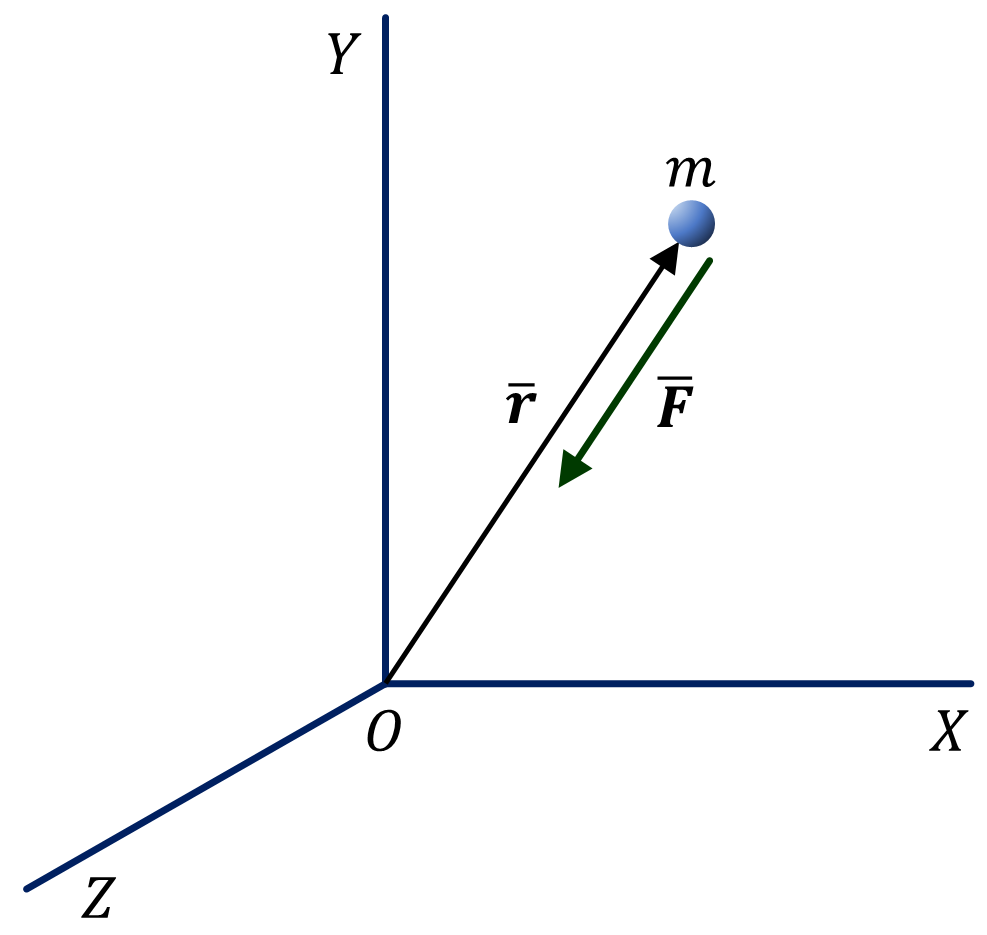
\includegraphics[width=0.36\textwidth]{figures/fig_restoring-force.png}
	\end{wrapfigure}
	A linear restoring force is one whose magnitude is linearly proportional to the displacement of a particle from a fixed reference point that is its \emph{mean position} of rest or equilibrium, and direction is opposite to the displacement.
	\resetwrappadding
	
	If a particle of mass $m$, which is at a point with position vector $\vb{r}$, is under the influence of a linear restoring force such that its mean position is the origin, then we have
	\begin{align}
		\vb{F}&\propto\qty(-\vb{r}) \nonumber\\
		\qq{or,}\vb{F}&=-k\vb{r} \label{eqn:restoring-force-01}
	\end{align}
	where $k$ is the proportionality constant, known as the \emph{force constant}.
	
	The linear restoring force is a conservative force and hence it has an associated potential energy field which can be obtained at an arbitrary point $\vb{r}$ as
	\begin{align}
		U(\vb{r})&=-\int\limits_{\infty}^{\vb{r}}{\vb{F}\cdot\dd{\vb{r}}} \label{eqn:U-restoring}
	\end{align}
	From equation (\ref{eqn:restoring-force-01}), we can write
	\begin{align*}
		\vb{F}&=-k\qty(x\vu{x}+y\vu{y}+z\vu{z})
	\end{align*}
	Also, we have that
	\begin{align*}
		\dd{\vb{r}}&=\vu{x}\dd{x}+\vu{y}\dd{y}+\vu{z}\dd{z}
	\end{align*}
	This gives us
	\begin{align*}
		\vb{F}\cdot\dd{\vb{r}}&=-k\qty(x\vu{x}+y\vu{y}+z\vu{z})\cdot\qty(\vu{x}\dd{x}+\vu{y}\dd{y}+\vu{z}\dd{z}) \\
		\implies\vb{F}\cdot\dd{\vb{r}}&=-k\qty(x\dd{x}+y\dd{y}+z\dd{z})
	\end{align*}
	Hence, in equation (\ref{eqn:U-restoring}), we have
	\begin{align}
		U(\vb{r})&=-\int\limits_{\infty}^{\vb{r}}{-k\qty(x\dd{x}+y\dd{y}+z\dd{z})} \nonumber\\
			&=k\qty[\int\limits_{\infty}^{x}{x\dd{x}} + \int\limits_{\infty}^{y}{y\dd{y}} + \int\limits_{\infty}^{z}{z\dd{z}}] \nonumber\\
			&=k\qty(\dfrac{x^2}{2}+\dfrac{y^2}{2}+\dfrac{z^2}{2})+C \nonumber\\
			&=\dfrac{1}{2}k\qty(x^2+y^2+z^2)+C \nonumber\\
		\implies U(\vb{r})&=\dfrac{1}{2}kr^2 + C \label{eqn:U-restoring-02}
	\end{align}
	where $C=k\qty[\dfrac{x^2}{2}+\dfrac{y^2}{2}+\dfrac{z^2}{2}]_{x,y,z\to\infty}$.
	
	If we choose the potential energy to be zero at the origin, i.e. $U=0$ at $\vb{r}=\vb{0}$, then from equation (\ref{eqn:U-restoring-02}), we obtain
	\begin{align*}
		0&=\dfrac{1}{2}k\times 0+C \\
		\implies C&=0
	\end{align*}
	
	\setwrappadding
	\begin{wrapfigure}[8]{r}{0.5\textwidth}
		\centering
		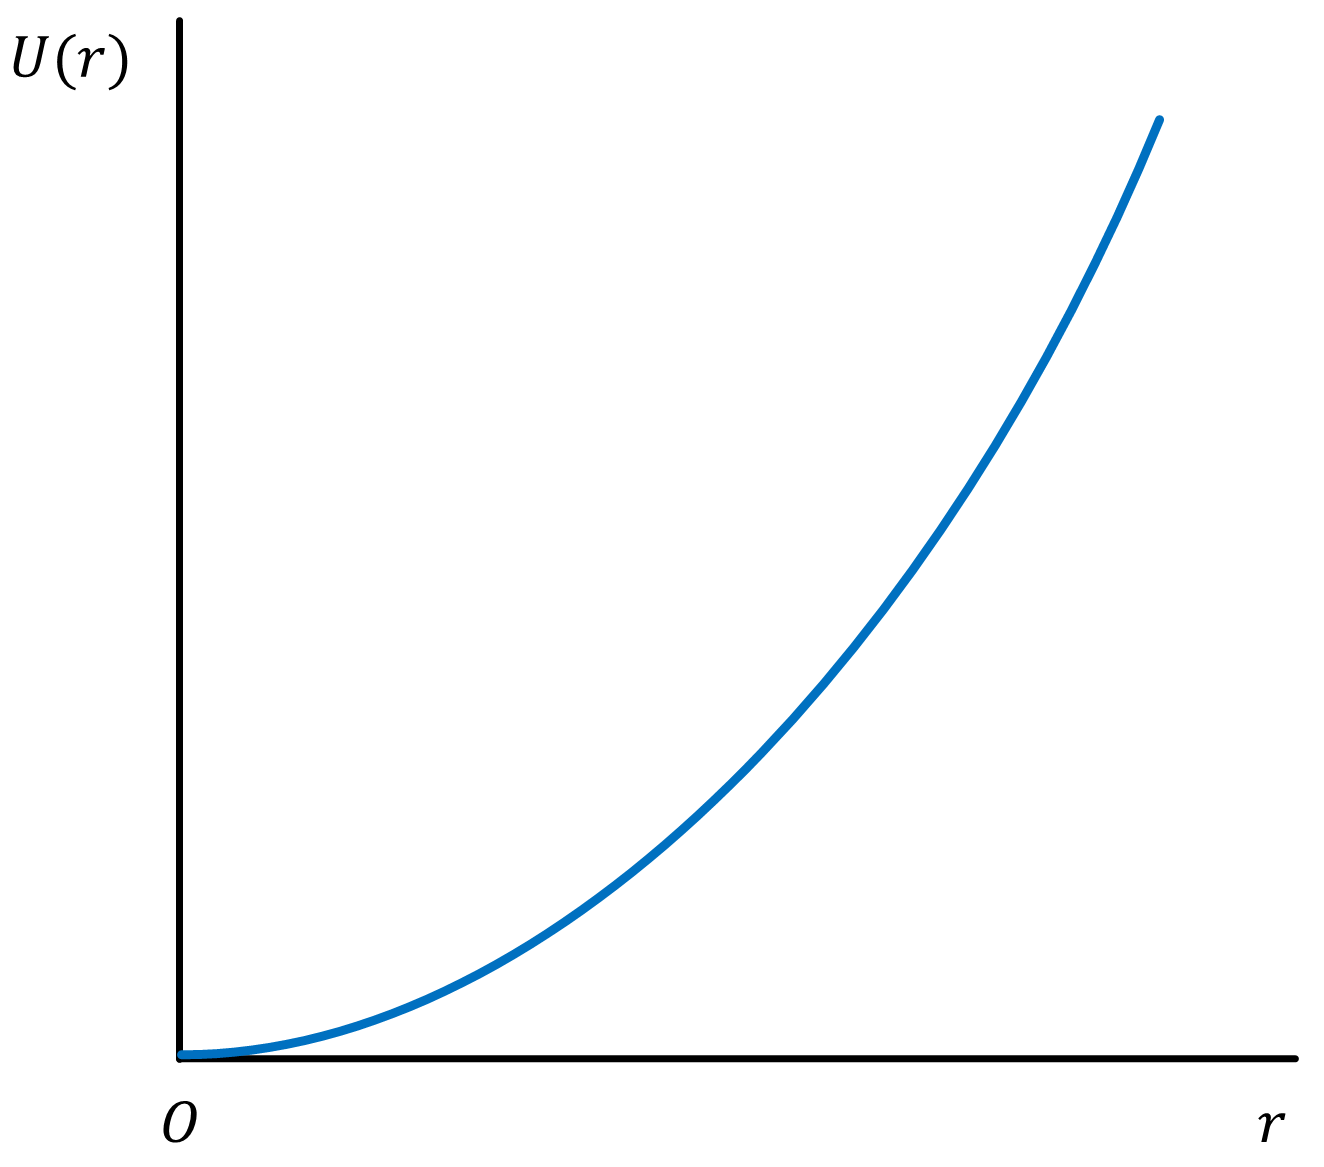
\includegraphics[width=0.48\textwidth]{figures/fig_restoring-potential-01.png}
	\end{wrapfigure}
	Then equation (\ref{eqn:U-restoring-02}) becomes
	\resetwrappadding
	\begin{align}
		\Aboxed{U(\vb{r})&=\dfrac{1}{2}kr^2} \label{eqn:U-restoring-03}
	\end{align}
	Equation (\ref{eqn:U-restoring-03}) shows that the potential energy due to a linear restoring force is a quadratic function of the distance of the particle from the mean position.
	
	\vspace{3.0cm}
	Suppose the motion of the particle is confined to the $X$-axis alone, i.e. $\vb{r}=x\vu{x}$ and hence $r^2=x^2$. Then the restoring force is
	\begin{align*}
		\vb{F}&=-kx\vu{x}
	\end{align*}
	The potential energy at any point on the $X$-axis is $U=\dfrac{1}{2}kx^2$.
	
	\begin{figure}[h!]
		\centering
		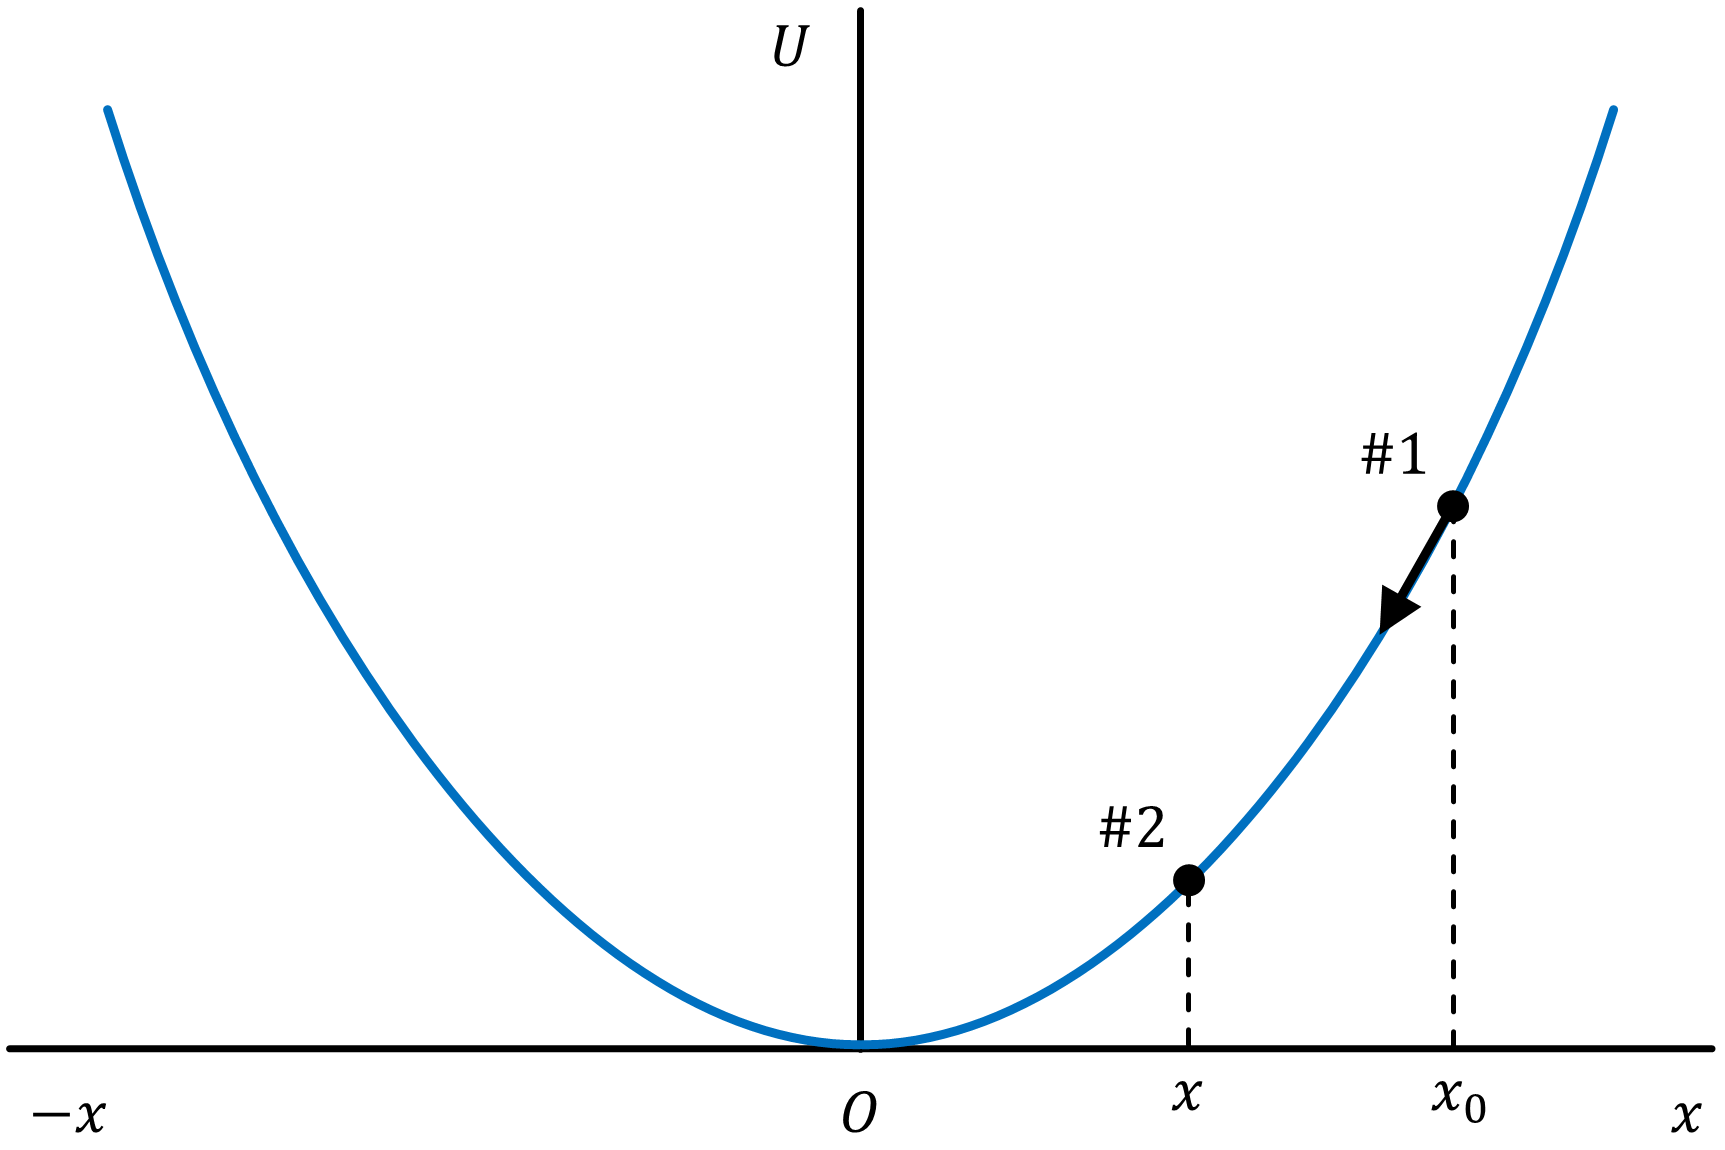
\includegraphics[width=0.6\textwidth]{figures/fig_restoring-potential-02.png}
	\end{figure}
	
	Let the particle be initially at the extreme position $x_0$ from the mean position at the origin, which corresponds to \#1 on the $U(x)$ plot. Then the initial potential energy at \#1 is
	\begin{align*}
		U_1&=\dfrac{1}{2}kx_0^2
	\end{align*}
	
	If the particle is released from position \#1 from rest, its initial kinetic energy is
	\begin{align*}
		T_1&=0
	\end{align*}
	
	Suppose that finally the particle reaches some arbitrary position $x$, which corresponds to \#2 on the $U(x)$ plot. Then the final potential energy is
	\begin{align*}
		U_2&=\dfrac{1}{2}kx^2
	\end{align*}
	
	Because at position \#2, the particle is in motion, its final kinetic energy is
	\begin{align*}
		T_2&=\dfrac{1}{2}mv^2
	\end{align*}
	
	Hence, the changes in its kinetic and potential energies are
	\begin{align*}
		\Delta T&=T_2-T_1=\dfrac{1}{2}mv^2-0=\dfrac{1}{2}mv^2 \\
		\Delta U&=U_2-U_1=\dfrac{1}{2}kx^2-\dfrac{1}{2}kx_0^2=\dfrac{1}{2}k\qty(x^2-x_0^2)
	\end{align*}
	
	Because the linear restoring force is conservative, we obtain from the law of conservation of mechanical energy that
	\begin{align}
		\Delta T+\Delta U&=0 \nonumber\\
		\implies\dfrac{1}{2}mv^2+\dfrac{1}{2}k\qty(x^2-x_0^2)&=0 \nonumber\\
		\implies v^2&=\dfrac{k}{m}\qty(x_0^2-x^2) \nonumber\\
		\implies \Aboxed{v&=\pm\sqrt{\dfrac{k}{m}\qty(x_0^2-x^2)}} \label{eqn:vel-restoring}
	\end{align}
	
	From Newton's second law of motion, we obtain the acceleration as
	\begin{align}
		F=ma&=-kx \nonumber\\
			\implies\Aboxed{a&=-\dfrac{k}{m}x} \label{eqn:acc-restoring}
	\end{align}
	
	\begin{itemize}
		\item When the particle is at the extreme positions at either side, i.e. $x=\pm x_0\implies x^2=x_0^2$, then we obtain from equation (\ref{eqn:vel-restoring}) that
		\begin{align*}
			v&=\pm\sqrt{\dfrac{k}{m}\qty(x_0^2-x_0^2)} \\
			\implies v&=0
		\end{align*}
		Also, from equation (\ref{eqn:acc-restoring}), we obtain
		\begin{align*}
			a=a_\text{max}&=-\dfrac{k}{m}x_0
		\end{align*}
		This means that the particle is at rest but under maximum magnitude of acceleration when it is at either of the extreme positions.
		
		\item When the particle is at the mean position, i.e. $x=0$, then we obtain from equation (\ref{eqn:vel-restoring}) that
		\begin{align*}
			v&=\pm\sqrt{\dfrac{k}{m}\qty(x_0^2-0)} \\
			\implies v=v_\text{max}&=\pm\sqrt{\dfrac{k}{m}x_0^2}
		\end{align*}
		And from equation (\ref{eqn:acc-restoring}), we obtain
		\begin{align*}
			a&=0
		\end{align*}
		This means that the particle moves with a maximum speed but under zero acceleration when it is at the mean positions.
	\end{itemize}
	
	The acceleration and velocities of the particle at the extreme positions, mean position and an arbitrary position are shown in the figure below.
	\begin{figure}[h!]
		\centering
		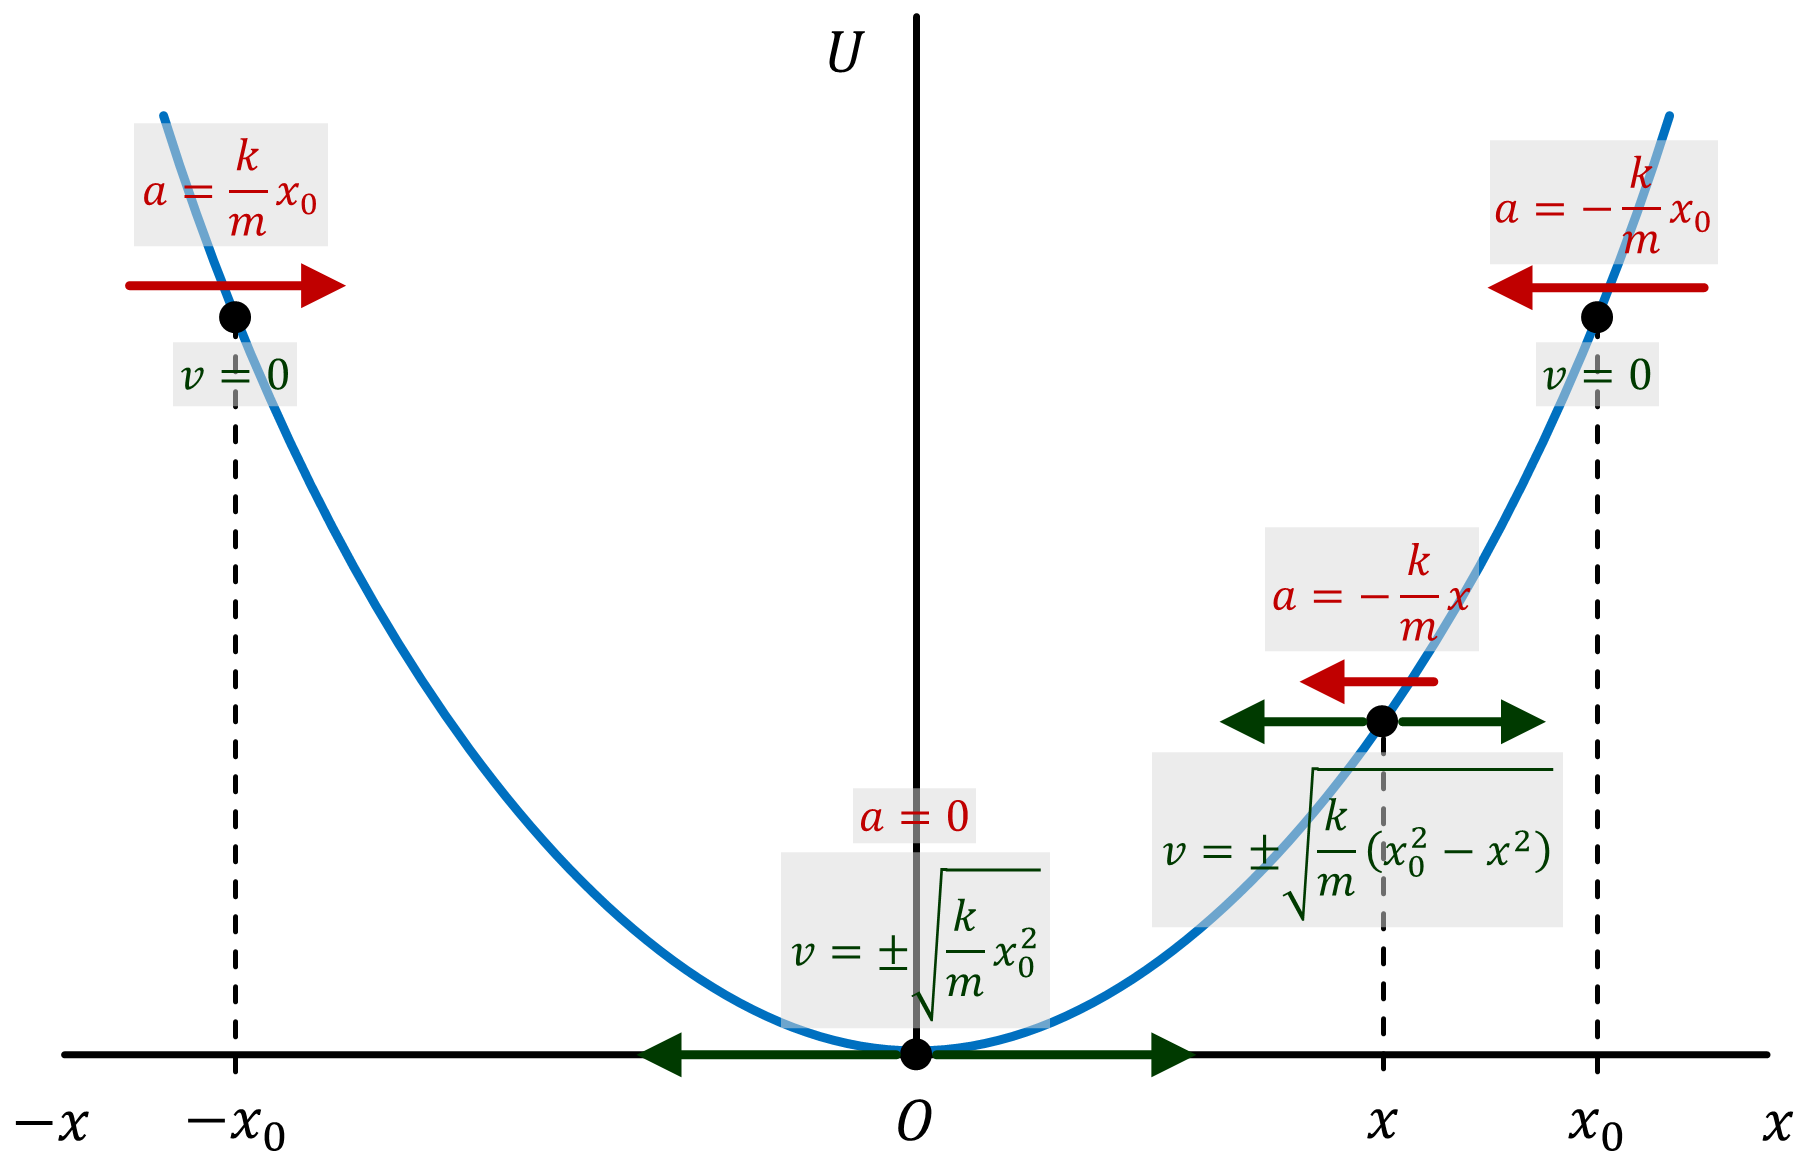
\includegraphics[width=0.7\textwidth]{figures/fig_restoring-potential-03.png}
	\end{figure}